\documentclass[12pt,letterpaper,oneside]{article}
\usepackage{setspace}
\usepackage{geometry}
\usepackage{graphicx}
\usepackage{url}
\usepackage{hyperref}

\hypersetup{
    colorlinks=true, %set true if you want colored links
    linktoc=all,     %set to all if you want both sections and s linked
    linkcolor=blue,  %choose some color if you want links to stand out
}
\usepackage{float}
\usepackage{amsmath}
\usepackage{booktabs}
\usepackage{color}
\usepackage{listings}
\usepackage{longtable}
\usepackage{listings}
\usepackage{color} %red, green, blue, yellow, cyan, magenta, black, white
\definecolor{mygreen}{RGB}{28,172,0} % color values Red, Green, Blue
\definecolor{mylilas}{RGB}{170,55,241}

\lstset{language=Matlab,%
    %basicstyle=\color{red},
    breaklines=true,%
    morekeywords={matlab2tikz},
    keywordstyle=\color{blue},%
    morekeywords=[2]{1}, keywordstyle=[2]{\color{black}},
    identifierstyle=\color{black},%
    stringstyle=\color{mylilas},
    commentstyle=\color{mygreen},%
    showstringspaces=false,%without this there will be a symbol in the places where there is a space
    numbers=left,%
    numberstyle={\tiny \color{black}},% size of the numbers
    numbersep=9pt, % this defines how far the numbers are from the text
    emph=[1]{for,end,break},emphstyle=[1]\color{red}, %some words to emphasise
    %emph=[2]{word1,word2}, emphstyle=[2]{style},    
}

\usepackage[parfill]{parskip}
\usepackage{chngcntr}
\usepackage[titletoc,toc,title]{appendix}

\renewcommand{\thesubsection}{3}

\usepackage{enumitem}
\usepackage[none]{hyphenat}
\usepackage{caption}
\usepackage{subcaption}
\counterwithin{figure}{section}
\counterwithin{table}{section}
\newcommand{\HRule}{\rule{\linewidth}{0.5mm}}
\geometry{letterpaper, portrait, margin=1in}
\pdfpagewidth=\paperwidth
\pdfpageheight=\paperheight
\DeclareGraphicsExtensions{.jpg,.png}

\begin{document}

%%%%%%%%%%%%%%%%%%%%%%%%%%%%%%%%%%%%%%%%%%%%%%%%%%%%%
%TITLEPAGE
\begin{titlepage}
\begin{center}
{\LARGE HDL Generator Documentation\\[1cm]}

\HRule \\[1.0cm]
{\LARGE \textsc{Author}\\[0.1cm]}
{\LARGE Wyatt Gronnemose\\[0.2cm]}

\thispagestyle{empty} %MAKES IT SO THAT THERE IS NO PAGE NUMBER
\clearpage
\end{center}
\end{titlepage}
%%%%%%%%%%%%%%%%%%%%%%%%%%%%%%%%%%%%%%%%%%%%%%%%%%%%

%STARTS PAGE NUMBER AT PAGE 2
\pagenumbering{roman}
\setcounter{page}{2}

%%%%%%%%%%%%%%%%%%%%%%%%%%%%%%%%%%%%%%%%%%%%%%%%%
%TABLE OF CONTENTS, LIST OF FIGURES, AND LIST OF TABLES
\newpage
\singlespacing

%%% TOC and document section numbering depth
\setcounter{tocdepth}{3}
\setcounter{secnumdepth}{3}

\tableofcontents
\listoffigures
\newpage
%%%%%%%%%%%%%%%%%%%%%%%%%%%%%%%%%%%%%%%%%%%%%%%%%%

%%%%%%%%%%%%%%%%%%%%%%%%%%%%%%%%%%%%%%%%%%%%%%%%%%
%STARTS THE BODY OF THE REPORT
\pagenumbering{arabic}
%\doublespacing
\flushleft

%%% reset section counters etc.
\setcounter{section}{0}
\setcounter{subsection}{0}
\setcounter{subsubsection}{0}

%%% display section, subsection, subsubsection numbering
\renewcommand{\thesection}{\arabic{section}}

\renewcommand{\thesubsection}{\arabic{section}.\arabic{subsection}}

\renewcommand{\thesubsubsection}{\arabic{section}.\arabic{subsection}.\arabic{subsubsection}}

% Input sections here
\section{Project Introduction}
\subsection{Purpose}
The purpose of this project is to be able to easily describe a state machine
and turn it into a hardware description language (HDL). The HDL can then be
used with FPGA's.

\subsection{System Architecture}
\begin{figure}[h]
   \centering
   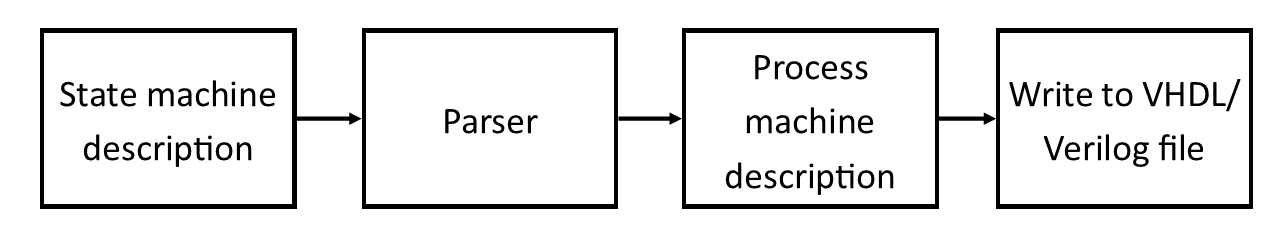
\includegraphics[scale=0.6]{SystemArchitecture}
   \caption{System Architecture}
   \label{fig:SysArchitecture}
\end{figure}


\section{Language Structure}
\label{sec:LanguageStructure}
This section defines how you express a state machine or system of state
machines. A Moore machine can be defined using a set of six items. These are:

\begin{itemize}
   \item Finite set of states (S)
   \item Initial state ($S_0$)
   \item Finite input alphabet ($\Sigma$)
   \item Finite ouitput alphabet ($\Lambda$)
   \item Transition function ($T:S\times\Sigma\rightarrow S$)
   \item Output function ($G:S \rightarrow \Lambda$)
\end{itemize}

Graphically this is shown below in Figure \ref{fig:MooreMachine}.

\begin{figure}[h]
   \centering
   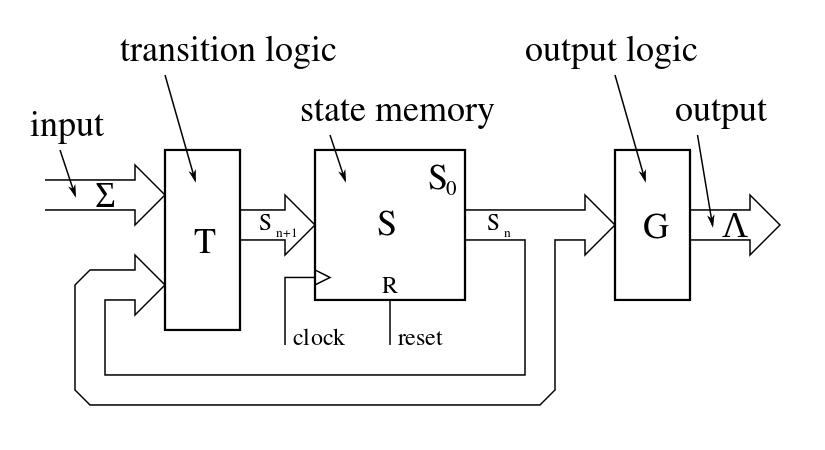
\includegraphics[scale=0.4]{MooreMachine}
   \caption{Moore Machine}
   \small{Taken from:://commons.wikimedia.org/wiki/File:Moore-Automat-en.svg}
   \label{fig:MooreMachine}
\end{figure}
\FloatBarrier

\subsection{State Machine Syntax}
The structure of a state machine is shown in the code below. It describes the
six parts of a Moore machine described in Section \ref{sec:LanguageStructure}
Language Structure.

\lstinputlisting{StateMachineExample.sm}

\subsection{System Syntax}


\end{document}

